%Version 3 December 2023
% See section 11 of the User Manual for version history
%
%%%%%%%%%%%%%%%%%%%%%%%%%%%%%%%%%%%%%%%%%%%%%%%%%%%%%%%%%%%%%%%%%%%%%%
%%                                                                 %%
%% Please do not use \input{...} to include other tex files.       %%
%% Submit your LaTeX manuscript as one .tex document.              %%
%%                                                                 %%
%% All additional figures and files should be attached             %%
%% separately and not embedded in the \TeX\ document itself.       %%
%%                                                                 %%
%%%%%%%%%%%%%%%%%%%%%%%%%%%%%%%%%%%%%%%%%%%%%%%%%%%%%%%%%%%%%%%%%%%%%

%%\documentclass[referee,sn-basic]{sn-jnl}% referee option is meant for double line spacing

%%=======================================================%%
%% to print line numbers in the margin use lineno option %%
%%=======================================================%%

%%\documentclass[lineno,sn-basic]{sn-jnl}% Basic Springer Nature Reference Style/Chemistry Reference Style

%%======================================================%%
%% to compile with pdflatex/xelatex use pdflatex option %%
%%======================================================%%

%%\documentclass[pdflatex,sn-basic]{sn-jnl}% Basic Springer Nature Reference Style/Chemistry Reference Style


%%Note: the following reference styles support Namedate and Numbered referencing. By default the style follows the most common style. To switch between the options you can add or remove “Numbered” in the optional parenthesis.
%%The option is available for: sn-basic.bst, sn-vancouver.bst, sn-chicago.bst%

%%\documentclass[pdflatex,sn-nature]{sn-jnl}% Style for submissions to Nature Portfolio journals
% \documentclass[pdflatex,sn-basic]{sn-jnl}% Basic Springer Nature Reference Style/Chemistry Reference Style
\documentclass[pdflatex,sn-mathphys-num]{sn-jnl}% Math and Physical Sciences Numbered Reference Style
% \documentclass[pdflatex,sn-mathphys-ay]{sn-jnl}% Math and Physical Sciences Author Year Reference Style
%%\documentclass[pdflatex,sn-aps]{sn-jnl}% American Physical Society (APS) Reference Style
%%\documentclass[pdflatex,sn-vancouver,Numbered]{sn-jnl}% Vancouver Reference Style
% \documentclass[pdflatex,sn-apa]{sn-jnl}% APA Reference Style
%%\documentclass[pdflatex,sn-chicago]{sn-jnl}% Chicago-based Humanities Reference Style

%%%% Standard Packages
%%<additional latex packages if required can be included here>

\usepackage{graphicx}%
\usepackage{multirow}%
\usepackage{amsmath,amssymb,amsfonts}%
\usepackage{amsthm}%
\usepackage{mathrsfs}%
\usepackage[title]{appendix}%
\usepackage{xcolor}%
\usepackage{textcomp}%
\usepackage{manyfoot}%
\usepackage{booktabs}%
\usepackage{algorithm}%
\usepackage{algorithmicx}%
\usepackage{algpseudocode}%
\usepackage{listings}%
\usepackage{subcaption}
\usepackage{hyperref}

\usepackage{colonequals}
\usepackage{tikz}
\usetikzlibrary{positioning}
\usetikzlibrary{automata}

\tikzset{%
  zeroarrow/.style = {-stealth,dashed},
  onearrow/.style = {-stealth,solid},
  c/.style = {circle,draw,solid,minimum width=2em,
        minimum height=2em},
  r/.style = {rectangle,draw,solid,minimum width=2em,
        minimum height=2em}
}

%%%%

%%%%%=============================================================================%%%%
%%%%  Remarks: This template is provided to aid authors with the preparation
%%%%  of original research articles intended for submission to journals published
%%%%  by Springer Nature. The guidance has been prepared in partnership with
%%%%  production teams to conform to Springer Nature technical requirements.
%%%%  Editorial and presentation requirements differ among journal portfolios and
%%%%  research disciplines. You may find sections in this template are irrelevant
%%%%  to your work and are empowered to omit any such section if allowed by the
%%%%  journal you intend to submit to. The submission guidelines and policies
%%%%  of the journal take precedence. A detailed User Manual is available in the
%%%%  template package for technical guidance.
%%%%%=============================================================================%%%%

%% as per the requirement new theorem styles can be included as shown below
\theoremstyle{thmstyleone}%
\newtheorem{theorem}{Theorem}%  meant for continuous numbers
%%\newtheorem{theorem}{Theorem}[section]% meant for sectionwise numbers
%% optional argument [theorem] produces theorem numbering sequence instead of independent numbers for Proposition
\newtheorem{proposition}[theorem]{Proposition}%
%%\newtheorem{proposition}{Proposition}% to get separate numbers for theorem and proposition etc.

\theoremstyle{thmstyletwo}%
\newtheorem{example}{Example}%
\newtheorem{remark}{Remark}%

\theoremstyle{thmstylethree}%
\newtheorem{definition}{Definition}%

\raggedbottom
% \unnumbered% uncomment this for unnumbered level heads

\begin{document}

\title[Article Title]{Mona Reimplemented: WS1S Logic with Mata}

%%=============================================================%%
%% GivenName	-> \fnm{Joergen W.}
%% Particle	-> \spfx{van der} -> surname prefix
%% FamilyName	-> \sur{Ploeg}
%% Suffix	-> \sfx{IV}
%% \author*[1,2]{\fnm{Joergen W.} \spfx{van der} \sur{Ploeg}
%%  \sfx{IV}}\email{iauthor@gmail.com}
%%=============================================================%%

\author{\fnm{Michal} \sur{Šedý}}\email{xsedym02@stud.fit.vutbr.cz}

%%==================================%%
%%     Unstructured abstract        %%
%%==================================%%

\abstract{This paper focuses on the reimplementation of the decision procedure for WS1S logic, a second-order logic that can be decided using finite automata. The well known tool for WS1S logic decision, Mona, employs automata with transitions represented through binary decision diagrams (BDDs). Due to the integration of BDDs in automata operations, tasks like reversal cannot be executed in the conventional manner of reverting individual edges. Instead, the reversal of each BDD must be computed, potentially resulting in an exponential blowup. Motivated by these limitations, Pavel Bednar reimplemented Mona using a pure automata approach with the Mata library. This work optimizes the automata methodology, resulting in a significant speedup, up to ten times faster, in WS1S decision compared to Bednar's original reimplementation.}


\keywords{Finite Automata, Binary Decision Diagrams, WS1S, MONA, MATA}


\maketitle


%%==================================%%
%%          INTRODUCTION            %%
%%==================================%%

\section{Introduction}
    The most well-known decision procedures are SAT and SMT \cite{SAT_SMT}, which are widely used in various applications such as verification (e.g., predicate abstraction), test generation, hardware synthesis, minimization, artificial intelligence, etc. The SAT (satisfiability) problem is a decision problem that asks whether a given propositional formula is satisfiable. The SMT (satisfiability modulo theories) problem extends the SAT problem to the satisfiability of first-order formulas with equality and atoms from various first-order theories. There are various higher-order decision procedures such as WS1S, WS2S, WSkS, S1S, etc.

    This work focuses on WS1S, the weak monadic second-order theory of the first successor. The term "weak" refers to finite sets, "monadic" indicates unary relations, "second-order" allows the usage of quantifiers over the relations, and "first successor" means that there is only one successor (e.g., the structure is linear).  WS1S \cite{WS1S} has an extremely simple syntax and semantics: it is variation of predicate logic with first-order variable that denote natural numbers and second-order variables that denote finite sets of natural numbers, it has a single function symbol, which denotes the successor function and has usual comparison operators such as $\leq$, $=$, $\in$ and $\supseteq$. Richard Büchi presented approach how to decide WS1S using finite automata in \cite{Buchi} The main idea is to recursively transform each subformula of the main WS1S formula into deterministic finite automata (DFA) representing feasible interpretations and simulate boolean operations via the automata operations.

    The most commonly used tool for deciding WS1S and WS2S is Mona\footnote{accessible at \url{https://www.brics.dk/mona/index.html}}, which employs Büchi's recursion approach for the construction of finite automata with binary decision diagrams (BDD) to represent all automaton transitions. The use of BDD makes the decision faster, but at the cost of making some automata operations, such as reversion, expensive (potentially resulting in exponential blowup). Despite this limitation, Mona is widely utilized in various fields of program verification, including the verification of programs with complex dynamic data structures \cite{DDS1, DDS2}, string analysis \cite{string_analysis}, parametrized systems \cite{parametrized_systems}, distributed systems \cite{distributed_systems}, automatic synthesis \cite{automatic_synthesis}, hardware verification \cite{hardware_verification}, and many others.

    The previously mentioned problem with hard-to-compute automata operations when using BDDs motivated Bc. Pavel Bednář's master's thesis \cite{Bednar}. He reimplemented Mona's decision of WS1S by using a pure automata-based approach with the Mata automata library\footnote{available at: \url{https://github.com/VeriFIT/mata}}. The special type of edge, the \textit{jumping edge} has been introduced. The jumping edge contains information about how many variables can be jumped over. The primary idea behind introducing the jumping edge was to enable jumps not only over inner states but also over automaton states, with no upper limit on the maximal jump. However, despite this innovation, the jumping edge did not yield significant improvements in terms of space or time compression. Furthermore, it appears that jumping edges led to an overcomplication of algorithms.

    In our approach, we reimplemented Bednář's solution by enhancing each automaton state with an index corresponding to the variable ID, mirroring the indexing strategy used for each inner node in the ordered BDD employed by Mona. This index information allows us to determine the length of a jump based on the indices of the source and destination states in the automaton's transition. Due to the indexing sequence on states follows a pattern of $0, 1, \dots, n-1, 0, 1, \dots, n-1, 0, \dots$, the longest jump can only reach to the next state with an index of $0$. While this might appear to be a step backward from Bednář's approach, the limitation on the jump length simplifies all algorithms. Surprisingly, it results in a significantly faster decision of the input formula, up to 10 times faster, compared to the variant with jumping edges.

    The first section introduces basic notations, definition of finite automata, binary decision diagrams, and WS1S. In the second section, we delve into the background of automata construction from WS1S formulas. The third section provides a detailed description of algorithms for intersection, union, complement, determinization, and minimization of automata with indexes. Moving to the fourth section, we present a~comparison of decision times between the Mona tool, automata with jumping edges, and automata with indexes. The experiments are divided into two parts. Initially, automata operations are tested separately on the automata generated during Mona computation. Following that, the comparison is executed on the entire input formula.

%%==================================%%
%%          INTRODUCTION            %%
%%==================================%%

\section{Preliminaries}
    In this section, we briefly introduce the definitions of nondeterministic and deterministic automata, binary decision diagrams, and the WS1S logic.

    \subsection{Automata}

        \begin{definition}
            A deterministic finite automaton is a 5-tuple $M = (Q, \Sigma, \delta, q_0, F)$, where its components are:
            \begin{itemize}[noindent]
                \item $Q$ is a finite nonempty set of states,
                \item $\Sigma$ is an alphabet,
                \item $\delta : Q \times \Sigma \rightarrow Q$ is a transition function,
                \item $q \in Q$ is an initial state, and
                \item $F \subseteq Q$ is a set of final states.
            \end{itemize}
        \end{definition}

        \begin{definition}
            A nondeterministic finite automaton is a 5-tuple $M = (Q, \Sigma, \delta, Q_0, F)$, where $Q$, $\Sigma$, and $F$ are defined identically as for the DFA. The transition function $\delta$~is defined as $\delta : Q \times \Sigma \rightarrow 2^{Q}$ and $Q_0 \subseteq Q$ is a nonempty set of initial states.
        \end{definition}

        Nondeterminism allows the automaton to make transitions to more than one successor based on the current state and the read input symbol. In contrast, its deterministic variant can transition to at most one state. Nondeterminism keeps the automaton more compact, but certain operations such as complementation cannot be performed directly on NFA. Therefore determinization is required beforehand.

    \subsection{Binary Decision Diagrams}
        Representation of the boolean function $\phi$ with $n$ logical variables leads to $2^n$ transitions for each automaton state in order to cover every possible combination of logical values. This exponential number of transitions can be reduced using Binary Decision Diagrams (BDDs). Binary Decision Diagrams provide a compact and, most importantly, canonical representation for logical functions in the form $\phi: \{0, 1\}^* \rightarrow \{0, 1\}$.

        \vspace*{0.5em}

        \begin{definition}
            The binary decision diagram \cite{BDD} is rooted, directed, connected, and acyclic graph defined as a 7-tuple $G = (N, T, var, low, high, root, val)$ where:
            \begin{itemize}[noindent]
                \item $N$ is finite set on non-terminal (inner) nodes,
                \item $T$ is a finite set of terminal nodes (leaves) such that $N \cap T = \emptyset$,
                \item $var : N \rightarrow N \cup T$ defines the low and high successors of the inner nodes,
                \item $root \in N \cup T$ is the root node, and
                \item $val : T \rightarrow \{0, 1\}$ assignes logical value to the leaves.
            \end{itemize}
        \end{definition}

        The size of the BDD is not determined only by the number of logical variables used within the function $\phi$ but also by the ordering of the variables in the BDD. The best variable ordering can result in a BDD with a linear (in the number of variables) number of nodes, while the worst ordering can lead to an exponential size.

        \begin{figure}[H]
            \centering
            \begin{subfigure}{0.5\textwidth}
                \includegraphics[width=1.2\textwidth]{Figures/BDD_Variable_Ordering_Bad.pdf}
            \end{subfigure}
            \hspace*{2cm}
            \begin{subfigure}{0.3\textwidth}
                \hspace*{1cm}
                \includegraphics[width=0.5\textwidth]{Figures/BDD_Variable_Ordering_Good.pdf}
            \end{subfigure}
            \caption{Two bdds for the function $f(x1,\dots, x_{2n}) = x_1x_2 + x_3x_4 + \cdots, x_{2n-1}x_{2n}$ with bad variable ordering (on the left) and good variable ordering (on the right).}
            \label{figure::ordering}
        \end{figure}

        Consider the Boolean function $f(x_1, \dots, x_{2n}) = x_1x_2 + x_3x_4 + \cdots + x_{2n-1}x_{2n}$. Using the variable ordering $x_1 < x_3 < \cdots < x_{2n-1} < x_2 < x_4 < \cdots < x_{2n}$, the Binary Decision Diagram (BDD) requires $2^{n+1}$ nodes to represent the function. Using the ordering $x_1 < x_2 < x_3 < x_4 < \cdots < x_{2n-1} < x_{2n}$, the BDD consists of $2n + 2$ nodes. An example of such orderings is shown in Figure \ref{figure::ordering}. The problem of finding the best variable ordering is NP-hard \cite{BDD_np-hard}. However, various heuristics exist to address this challenge \cite{BDD_heuristics}.

        \vspace*{0.5em}

        \begin{definition}
            Let $\prec$ be a given ordering on logical variables $Var$, a Binary Decision Diagram (BDD) $G$ is ordered (OBDD) with respect to $\prec$ if, for every $n \in \mathbb{N}$, the following conditions hold:
            \begin{enumerate}[noindent]
                \item $low(n) \in N \implies var(n) \prec var(low(n))$
                \item $high(n) \in N \implies var(n) \prec var(high(n))$
            \end{enumerate}
        \end{definition}

        \begin{definition}
            The OBDD $G = (N, T, var, low, high, root, val)$ is a Reduced OBDD (ROBDD) if the following conditions are satisfied:
            \begin{enumerate}[noindent]
                \item $\forall t_1, t_2 \in T : val(t_1) \neq val(t_2)$
                \item There are no isomorphic subgraphs in $G$
                \item $\forall n_1, n_2 \in N : low(n_1) \neq low(n_2) \lor high(n_1) \neq high(n_2)$
            \end{enumerate}
        \end{definition}

        \begin{figure}[H]
            \centering
            \begin{subfigure}{0.45\textwidth}
                \centering
                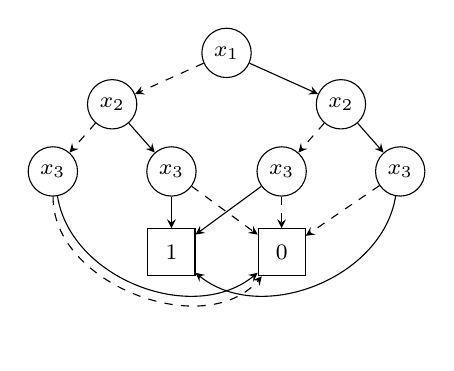
\begin{tikzpicture}[node distance=0.4cm and 0.3cm]\footnotesize
                    \node[c] (x1) {$x_1$};
                    \node[c] (x2a) [below left=0.2cm and 1cm of x1] {$x_2$};
                    \node[c] (x2b) [below right=0.2cm and 1cm of x1] {$x_2$};
                    \node[c] (x3a) [below left=of x2a] {$x_3$};
                    \node[c] (x3b) [below right=of x2a] {$x_3$};
                    \node[c] (x3c) [below left=of x2b] {$x_3$};
                    \node[c] (x3d) [below right=of x2b] {$x_3$};
                    \node[r] (one) [below=of x3b] {1};
                    \node[r] (zero) [below=of x3c] {0};

                    \draw[onearrow] (x1) -- (x2b);
                    \draw[onearrow] (x2a) -- (x3b);
                    \draw[onearrow] (x2b) -- (x3d);
                    \draw[onearrow] (x3a) to[bend right=60] (zero);
                    \draw[onearrow] (x3b) -- (one);
                    \draw[onearrow] (x3c) -- (one);
                    \draw[onearrow] (x3d) to[bend left=60] (one);

                    \draw[zeroarrow] (x1) -- (x2a);
                    \draw[zeroarrow] (x2a) -- (x3a);
                    \draw[zeroarrow] (x2b) -- (x3c);
                    \draw[zeroarrow] (x3a) to[bend right=70] (zero);
                    \draw[zeroarrow] (x3b) -- (zero);
                    \draw[zeroarrow] (x3c) -- (zero);
                    \draw[zeroarrow] (x3d) -- (zero);
                 \end{tikzpicture}
            \end{subfigure}
            \begin{subfigure}{0.25\textwidth}
                \centering
                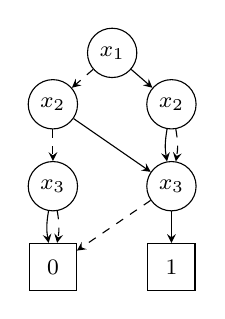
\begin{tikzpicture}[node distance=0.4cm and 0.3cm]\footnotesize
                    \node[c] (x1) {$x_1$};
                    \node[c] (x2a) [below left=0.2cm and 0.3cm of x1] {$x_2$};
                    \node[c] (x2b) [below right=0.2cm and 0.3cm of x1] {$x_2$};
                    \node[c] (x3a) [below=of x2a] {$x_3$};
                    \node[c] (x3b) [below=of x2b] {$x_3$};
                    \node[r] (one) [below=of x3b] {1};
                    \node[r] (zero) [below=of x3a] {0};

                    \draw[onearrow] (x1) -- (x2b);
                    \draw[onearrow] (x2a) -- (x3b);
                    \draw[onearrow] (x2b) to[bend right=10] (x3b);
                    \draw[onearrow] (x3a) to[bend right=10] (zero);
                    \draw[onearrow] (x3b) -- (one);

                    \draw[zeroarrow] (x1) -- (x2a);
                    \draw[zeroarrow] (x2a) -- (x3a);
                    \draw[zeroarrow] (x2b) to[bend left=10] (x3b);
                    \draw[zeroarrow] (x3a) to[bend left=10] (zero);
                    \draw[zeroarrow] (x3b) -- (zero);
                 \end{tikzpicture}
            \end{subfigure}
            \begin{subfigure}{0.25\textwidth}
                \centering
                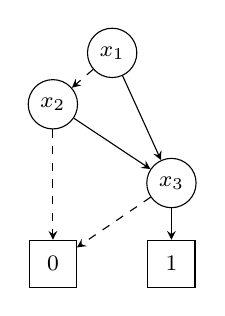
\begin{tikzpicture}[node distance=0.4cm and 0.3cm]\footnotesize
                    \node[c] (x1) {$x_1$};
                    \node[c] (x2) [below left=0.2cm and 0.3cm of x1] {$x_2$};
                    \node[c] (x3) [below right=1.2cm and 0.3cm of x1] {$x_3$};
                    \node[r] (one) [below=of x3] {1};
                    \node[r] (zero) [below= 1.4cm of x2] {0};

                    \draw[onearrow] (x1) -- (x3);
                    \draw[onearrow] (x2) -- (x3);
                    \draw[onearrow] (x3) -- (one);

                    \draw[zeroarrow] (x1) -- (x2);
                    \draw[zeroarrow] (x2) -- (zero);
                    \draw[zeroarrow] (x3) -- (zero);
                 \end{tikzpicture}
            \end{subfigure}
            \caption{From left to right, an OBDD satisfies the first, second, and third conditions as specified in the definition of ROBDD.}
        \end{figure}

        \vspace*{-1em}

        \begin{theorem}
            \label{theorem:ROBDD}
            For every Boolean function $\phi$ over some set of variables $Var$ and every variable ordering $\prec$ on $Var$, there is a unique (up to isomorphism) reduced OBDD (with respect to $\prec$) $G_\phi$ which represents $\phi$. \cite{BDD}"
        \end{theorem}

        \vspace*{0.5em}

        Based on Theorem \ref{theorem:ROBDD}, checking the equivalence of two functions, $\phi_1$ and $\phi_2$, represented by Reduced OBDDs (ROBDDs) $G_1$ and $G_2$ is equivalent to checking the isomorphism of $G_1$ and $G_2$.

        Moreover, if several Boolean functions are represented with one shared ROBDD with multiple roots, as Mona does, the equivalence checking is reduced from isomorphism checking to simply checking the identity of the BDD roots.


    \subsection{WS1S}
        Richard Büchi showed that WS1S is equivalent to regular expressions and can therefore be represented by finite automata \cite{Buchi}. In this subsection, the simplification of the WS1S formula and its semantics will be presented, followed by the transformation of atomic formulae to automata. The main source for this subsection was \cite{Mona_manual}.

        \subsubsection*{Formula simplification}
            First-order terms are encoded as second-order terms since a first-order value can be seen as a singleton second-order value. Also, booleans can be encoded using the first position in the input automaton string.

            All second-order terms are 'flattened' by introducing new variables that contain the values of all subterms. For example, the formula $A = (B \cup C) \cap D$ will be transformed into the form $\exists V : A = V \cap D \land V = B \cup C$, where $V$ is a new variable.

            Subformulae are simplified to contain fewer operators. As a result, only basic operations have to be implemented by the solver. The abstract syntax for simplified WS1S formulas can be defined by the following grammar:
            $$
                \phi \colonequals \neg \phi' | \phi' \land \phi'' | \exists P_i : \phi' | P_i \subseteq P_j | P_i = P_j \setminus P_k | P_i = P_j + 1
            $$

        \subsubsection*{Semantic}
            Given the main formula $\phi_0$, we define its semantic inductively relative to a string $w$ over the alphabet $\mathbb{B}^k$, where $\mathbb{B} = {0, 1}$ and $k$ is the number of variables in $\phi_0$. Assume every variable of $\phi_0$ is assigned a unique number in the range $1, 2, \dots, k$, called the \textit{variable index}. The string $w$ now determines an interpretation $w(P_i)$ of $P_i$, defined as the finite set ${j ,|, \text{the } j\text{th bit in the } P_i\text{-track is 1}}$. For example, the formula $\phi_0 \equiv \exists C : A = B \setminus C$ has variables $A$, $B$, and $C$, which are assigned the indices 1, 2, and 3, respectively. A typical string $w$ over $\mathbb{B}^3$ looks like:

            $$
            \begin{matrix}
                A\\
                B\\
                C
            \end{matrix}
            \hspace*{2em}
            \begin{pmatrix}
                1\\
                0\\
                1
            \end{pmatrix}
            \begin{pmatrix}
                0\\
                0\\
                1
            \end{pmatrix}
            \begin{pmatrix}
                1\\
                1\\
                0
            \end{pmatrix}
            \begin{pmatrix}
                0\\
                0\\
                0\\
            \end{pmatrix}
            $$

            \vspace*{0.5em}

            \noindent It's important to note that $w$ with the suffix $(0^*)^T$ defines the same interpretation as $w$. Therefore, the minimum $w$ is such a string that there is no such non-empty suffix. The semantics of a formula $\phi$ is defined inductively:
                \begin{alignat*}{2}
                    &w \vDash \neg \phi' \quad && \textnormal{iff}\quad  w \nvDash \phi'\\
                    &w \vDash \phi' \land \phi'' \quad &&\textnormal{iff}\quad  w \vDash \phi' \land w \vDash \phi''\\
                    &w \vDash \exists P_i : \phi' \quad &&\textnormal{iff}\quad  \exists finite(M) \subseteq \mathbb{N} : w[P_i \mapsto M] \vDash \phi'\\
                    &w \vDash P_i \subseteq P_j \quad &&\textnormal{iff}\quad  w(P_i) \subseteq w(P_j)\\
                    &w \vDash P_i = P_j \setminus P_k \quad &&\textnormal{iff}\quad  w(P_i) = w(P_j) \setminus w(P_k)\\
                    &w \vDash P_i = P_j + 1 \quad &&\textnormal{iff}\quad  w(P_i) = \{j + 1\,|\, j \in w(P_j)\}
                \end{alignat*}

                where we use the notation $w[P_i \mapsto M]$ for the shortest string $w'$ that interprets all variables $P_j$, $j \neq i$, as $w$ does but interprets $P_i$ as $M$. Note that if we assume that $w$ is minimum, then $w'$ decomposes into $w' = w \cdot w''$, where $w''$ is a string of letters of the form $(0^*X0^*)^T$, and the $i$th component is the only one that may be different from 0.

        \subsubsection*{Automaton construction}
            The input formula $\phi$ is recursively transformed into the deterministic finite automaton that represents the set of satisfying strings $L(\phi) = {w,|, w \vDash \phi}$. The translation of atomic and composite formulae to deterministic finite automata follows:


            \vspace*{0.5em}

            \begin{itemize}
                \item $\phi = P_1 \subseteq P_2$:
                    \begin{figure}[H]
                        \centering
                        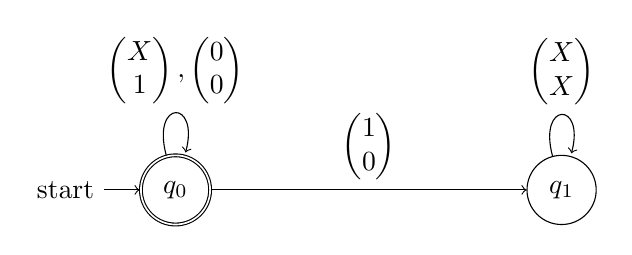
\begin{tikzpicture}
                            \centering
                            \node[state, initial, accepting] (q0) {$q_0$};
                            \node[state] (q1) [right=4cm of q0]{$q_1$};

                            \path[->] (q0) edge node[above] {$\begin{pmatrix}1\\0\end{pmatrix}$} (q1)
                                    (q0) edge[loop above] node {$\begin{pmatrix}X\\1\end{pmatrix},\begin{pmatrix}0\\0\end{pmatrix}$} ()
                                    (q1) edge[loop above] node {$\begin{pmatrix}X\\X\end{pmatrix}$} ();
                        \end{tikzpicture}
                    \end{figure}
                \vspace*{0.5em}
                \item $\phi = P_1 = P_2 \setminus P_3$:
                    \begin{figure}[H]
                        \centering
                        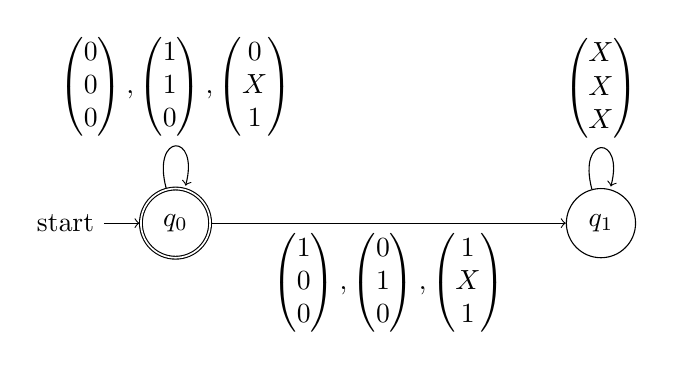
\begin{tikzpicture}
                            \centering
                            \node[state, initial, accepting] (q0) {$q_0$};
                            \node[state] (q1) [right=4.5cm of q0]{$q_1$};

                            \path[->] (q0) edge node[below] {$\begin{pmatrix}1\\0\\0\end{pmatrix},\begin{pmatrix}0\\1\\0\end{pmatrix},\begin{pmatrix}1\\X\\1\end{pmatrix}$} (q1)
                                    (q0) edge[loop above] node {$\begin{pmatrix}0\\0\\0\end{pmatrix},\begin{pmatrix}1\\1\\0\end{pmatrix},\begin{pmatrix}0\\X\\1\end{pmatrix}$} ()
                                    (q1) edge[loop above] node {$\begin{pmatrix}X\\X\\X\end{pmatrix}$} ();
                        \end{tikzpicture}
                    \end{figure}
                \newpage
                \item $\phi = P_1 = P_2 + 1$:
                    \vspace*{-1em}
                    \begin{figure}[H]
                        \centering
                        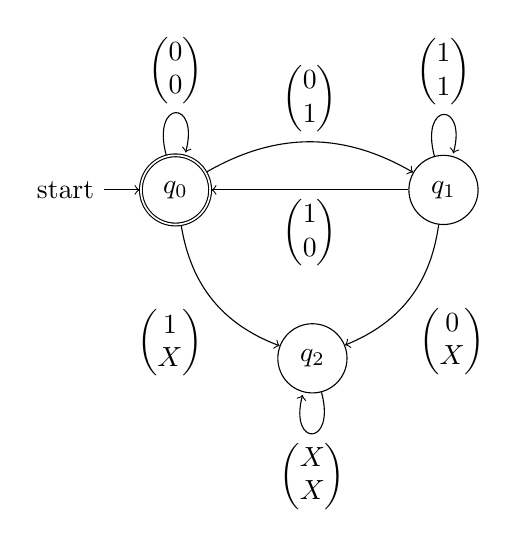
\begin{tikzpicture}
                            \centering
                            \node[state, initial, accepting] (q0) {$q_0$};
                            \node[state] (q1) [right=2.5cm of q0]{$q_1$};
                            \node[state] (q2) [below right=1.5cm and 1.1cm of q0] {$q_2$};
                            \path[->] (q0) edge[bend left] node[above] {$\begin{pmatrix}0\\1\end{pmatrix}$} (q1)
                                      (q0) edge[loop above] node[above] {$\begin{pmatrix}0\\0\end{pmatrix}$} ()
                                      (q0) edge[bend right] node[below left] {$\begin{pmatrix}1\\X\end{pmatrix}$} (q2)
                                      (q1) edge[bend left] node[below right] {$\begin{pmatrix}0\\X\end{pmatrix}$} (q2)
                                      (q1) edge node[below] {$\begin{pmatrix}1\\0\end{pmatrix}$} (q0)
                                      (q1) edge[loop above] node[above] {$\begin{pmatrix}1\\1\end{pmatrix}$} ()
                                      (q2) edge[loop below] node[below] {$\begin{pmatrix}X\\X\end{pmatrix}$} ();
                        \end{tikzpicture}
                    \end{figure}
                \item $\phi = \neg \phi'$: Negation of a formula corresponds to automaton complementation. If we have already calculated $A'$ such that $L(\phi') = L(A')$, then $L(\neg \phi') = \complement L(\phi') = \complement L(A') = L(\complement A')$, where $\complement$ denotes both language complementation and automata complementation. If the automaton is complete and deterministic, then complementation can be done by swapping accepting and non-accepting states.
                \vspace*{0.5em}
                \item $\phi = \phi' \land \phi''$: Conjunction corresponds to language intersection, $L(\phi' \land \phi'') = L(\phi') \cap L(\phi'')$. So, the resulting automaton $A$ is obtained by the production of automata $A' \times A''$, where $L(\phi') = L(A')$ and $L(\phi'') = L(A'')$.
                \vspace*{0.5em}
                \item $\phi = \exists P_i : \phi'$:  Intuitively, the desired automaton $A$ acts as the automaton $A'$ for $\phi'$ except that it is allowed to guess the bits on the $P_i$-track. The resulting automaton $A$ is nondeterministic. It is necessary to apply determinization and adjust the automaton $A$ in such a way that each $w \in L(A)$ is minimal.
            \end{itemize}



\section{Automata representation}
    \subsection{Mona}
    \subsection{Automata with Jumping Edges}
    \subsection{Automata with Indexed States}
        \begin{definition}
            Let $M = (Q, \Sigma, \delta, Q_0, F)$ be an NFA. The automaton $M$ is called an automaton with indexing if there exists an index function $\iota : Q \rightarrow \mathbb{N}_0$ such that the following conditions hold:
            \begin{enumerate}[noindent]
                \item $\forall q \in Q_0 : \iota(q) = 0$
                \item $\forall q \in F : \iota(q) = 0$
                \item $\forall q, r \in Q : \nexists a \in \Sigma : r \in \delta(q, a) \land \iota(r) \neq 0 \land \iota(q) \geq \iota(r)$
            \end{enumerate}
        \end{definition}

        The first and second conditions reflect the fact that only roots or leaves in the BDD can be initial and final states, respectively. The third condition demands that the part of the automaton simulating the BDD must be acyclic, with the exception of the root nodes/states with index 0.

\section{Automata operations}
    \subsection{Complement}
    \subsection{Union}
    \subsection{Intersection}
    \subsection{Determinization}
    \subsection{Minimization}
    \subsection{Projection}

\section{Experimental results}
    \subsection{Operations performance}
    \subsection{WS1S formulae}

\section{Conclusion}




% \begin{appendices}

% \section{Section title of first appendix}\label{secA1}

% An appendix contains supplementary information that is not an essential part of the text itself but which may be helpful in providing a more comprehensive understanding of the research problem or it is information that is too cumbersome to be included in the body of the paper.

% %%=============================================%%
% %% For submissions to Nature Portfolio Journals %%
% %% please use the heading ``Extended Data''.   %%
% %%=============================================%%

% %%=============================================================%%
% %% Sample for another appendix section			       %%
% %%=============================================================%%

% %% \section{Example of another appendix section}\label{secA2}%
% %% Appendices may be used for helpful, supporting or essential material that would otherwise
% %% clutter, break up or be distracting to the text. Appendices can consist of sections, figures,
% %% tables and equations etc.

% \end{appendices}

%%===========================================================================================%%
%% If you are submitting to one of the Nature Portfolio journals, using the eJP submission   %%
%% system, please include the references within the manuscript file itself. You may do this  %%
%% by copying the reference list from your .bbl file, paste it into the main manuscript .tex %%
%% file, and delete the associated \verb+\bibliography+ commands.                            %%
%%===========================================================================================%%

\bibliography{sn-bibliography}% common bib file
%% if required, the content of .bbl file can be included here once bbl is generated
%%\input sn-article.bbl


\end{document}
